\vspace{-3pt}
\section{实验结果}
\label{sec:experimental_results}

\begin{table*}[t]
\centering
\resizebox{\textwidth}{!}{
\begin{tabular}{l|cccc|cccc|cccc|cccc}
\toprule
\multirow{2}{*}{\textbf{Methods}} & \multicolumn{4}{c|}{\textbf{MPReID}} & \multicolumn{4}{c|}{\textbf{HMReID}} & \multicolumn{4}{c|}{\textbf{GibsonReID}} & \multicolumn{4}{c}{\textbf{ReplicaReID}} \\
 & Accuracy & Precision & Recall & F1 & Accuracy & Precision & Recall & F1 & Accuracy & Precision & Recall & F1 & Accuracy & Precision & Recall & F1 \\
\midrule
CVNet & 17.45 & 29.52 & 17.45 & 19.34 & 11.71 & 25.42 & 11.95 & 13.86 & 12.04 & 24.06 & 12.07 & 14.27 & 15.93 & 20.53 & 15.74 & 16.64 \\
DINOv2 & 59.36 & 64.68 & 59.36 & 58.91 & 53.91 & 60.52 & 53.73 & 54.69 & 61.01 & 65.88 & 61.78 & 61.71 & 78.06 & 79.68 & 77.97 & 77.44 \\
Patch-NetVLAD & 64.32 & 70.47 & 64.36 & 65.53 & 64.86 & 68.78 & 64.32 & 65.16 & 61.47 & 66.90 & 62.04 & 62.51 & 63.77 & 64.97 & 63.86 & 63.87 \\
AnyLoc & 92.34 & 93.23 & 92.36 & 92.32 & 89.69 & 90.25 & 89.53 & 89.62 & 85.85 & 87.42 & 86.15 & 86.21 & \textbf{88.57} & \textbf{89.89} & \textbf{88.46} & \textbf{88.42} \\
\rowcolor{Lavender}
AirRoom & \textbf{93.96} & \textbf{94.52} & \textbf{93.98} & \textbf{93.91} & \textbf{93.80} & \textbf{94.01} & \textbf{93.55} & \textbf{93.62} & \textbf{91.68} & \textbf{92.41} & \textbf{91.79} & \textbf{91.63} & 87.18 & 89.39 & 87.08 & 87.24 \\
\bottomrule
\end{tabular}
}
\vspace{-5pt}
\caption{AirRoom 与基线模型在四个新构建的房间重识别数据集上的整体性能对比。}
\vspace{-12pt}
\label{tab:overall}
\end{table*}
\subsection{数据集}
\vspace{-5pt}
目前没有现有的室内场景数据集完全适用于房间再识别任务,因为没有一个数据集能完全满足要求。像 ScanNet++ \cite{yeshwanth2023scannethighfidelitydataset3d} 和 MIT Indoor Scenes \cite{5206537} 这样的数据集缺乏房间级别的分割,导致多个房间共享一个场景标签。17 Places \cite{7801503} 数据集包含了唯一标签的房间,但视角变化有限,而且图像往往较为模糊。尽管该数据集也包含昼夜变化,但这些变化对于大多数室内场景并不特别相关。Reloc110 \cite{aryan2023airlocobjectbasedindoorrelocalization} 数据集可能是最合适的选择;然而,它的质量不够理想,许多图像仅包含纯色的墙壁或地板,由于随机采样,导致上下文信息非常少。

一些高质量的室内 3D 数据集——如 Matterport3D \cite{Matterport3D}、Habitat-Matterport3D \cite{ramakrishnan2021hm3d}、Gibson Database of 3D Spaces \cite{xiazamirhe2018gibsonenv} 和 Replica \cite{replica19arxiv}——提供了真实世界的室内场景。基于这些资源,并利用互动式 Habitat Simulator \cite{puig2023habitat3, szot2021habitat, habitat19iccv},我们创建了四个新的数据集:MPReID、HMReID、GibsonReID 和 ReplicaReID,如 \fref{fig:dataset_image} 所示。

使用 Habitat Simulator,我们为每个房间配置了一个代理,并手动选择了 5 到 10 个关键姿势来引导其探索。代理从不同角度捕捉了 640×480 的 RGB-D 图像,每个房间的图像数量为 300 到 800 张,具体取决于关键姿势的数量。然而,许多随机采样的图像质量较差,通常只包含墙壁或地板,缺乏足够的上下文信息。为了解决这一问题,我们仔细筛选了每个房间的图像,保留了那些准确代表空间并为房间 ReID 提供有价值信息的图像。

总的来说,这些数据集如下:MPReID 包括 15 个场景、105 个房间和 16,231 张 RGB-D 图像;HMReID 包含 21 个场景、105 个房间和 15,781 张 RGB-D 图像;GibsonReID 包含 24 个场景、45 个房间和 6,743 张 RGB-D 图像;ReplicaReID 包括 12 个场景、19 个房间和 2,862 张 RGB-D 图像。

\vspace{-4pt}
\subsection{数据库预处理}
\vspace{-4pt}

在房间重识别设置中,我们有多个查询图像和一个参考数据库。对于每个数据集,我们仅选择每个房间的一张图像来构建数据库。具体来说,对于每个房间的所有图像,我们首先使用 CLIP \cite{radford2021learningtransferablevisualmodels} 提取特征嵌入。然后,我们应用 K-means 聚类,设定聚类数为 1。距离聚类中心最近的图像被选择为参考图像,因为它最能代表房间的视觉特征 \cite{tan2005introduction}。

在构建参考数据库后,我们对特征进行预处理。首先,我们使用全局特征提取器来获取并保存全局上下文特征。接着,我们应用实例分割模块对物体进行分割。然后,我们使用我们的感受野扩展器来获取物体补丁,并使用物体特征提取器来提取并保存物体和补丁的特征。

\vspace{-4pt}
\subsection{实验概述}
\vspace{-4pt}
我们进行了五个主要实验:整体性能比较、分组性能比较、管道灵活性评估、消融研究和运行时分析。在评估过程中,我们使用了准确率、精确度、召回率和F1分数作为评价指标。每个类别的精确度、召回率和F1分数是通过多类混淆矩阵计算得出的,随后进行了宏平均。准确率是通过正确匹配的查询与总查询数之比来衡量的。详细的运行时分析和其他实验结果在附录中提供。

\begin{table*}[t]
\centering
\resizebox{\textwidth}{!}{
\begin{tabular}{l|cccc|cccc|cccc|cccc}
\toprule
\multirow{2}{*}{\textbf{Methods}} & \multicolumn{4}{c|}{\textbf{MPReID}} & \multicolumn{4}{c|}{\textbf{HMReID}} & \multicolumn{4}{c|}{\textbf{GibsonReID}} & \multicolumn{4}{c}{\textbf{ReplicaReID}} \\
 & Accuracy & Precision & Recall & F1 & Accuracy & Precision & Recall & F1 & Accuracy & Precision & Recall & F1 & Accuracy & Precision & Recall & F1 \\
\midrule
ResNet50 & 76.14 & 79.21 & 76.20 & 76.58 & 69.03 & 73.21 & 68.61 & 69.07 & 68.84 & 72.30 & 69.50 & 69.00 & 75.05 & 78.61 & 75.30 & 74.88 \\
CVNet & 17.45 & 29.52 & 17.45 & 19.34 & 11.71 & 25.42 & 11.95 & 13.86 & 12.04 & 24.06 & 12.07 & 14.27 & 15.93 & 20.53 & 15.74 & 16.64 \\
\rowcolor{Lavender}
AirRoom-ResNet50 & \textbf{86.16} & \textbf{87.69} & \textbf{86.19} & \textbf{86.16} & \textbf{81.23} & \textbf{83.90} & \textbf{80.76} & \textbf{81.23} & \textbf{82.53} & \textbf{84.91} & \textbf{82.86} & \textbf{82.54} & \textbf{83.51} & \textbf{84.85} & \textbf{83.54} & \textbf{83.17} \\
\cdashline{1-17}
NetVLAD & 82.22 & 86.77 & 82.24 & 82.92 & 72.04 & 80.79 & 71.83 & 73.05 & 68.86 & 81.00 & 69.24 & 71.01 & 77.04 & 81.31 & 77.28 & 77.63 \\
Patch-NetVLAD(4096) & 64.32 & 70.47 & 64.36 & 65.53 & 64.86 & 68.78 & 64.32 & 65.16 & 61.47 & 66.90 & 62.04 & 62.51 & 63.77 & 64.97 & 63.86 & 63.87 \\
Patch-NetVLAD(512) & 66.62 & 71.85 & 66.67 & 67.62 & 65.63 & 69.28 & 65.01 & 65.57 & 60.95 & 69.16 & 61.43 & 62.46 & 66.00 & 68.75 & 66.25 & 66.22 \\
Patch-NetVLAD(128) & 65.04 & 70.84 & 65.09 & 66.15 & 61.17 & 66.71 & 60.69 & 61.42 & 58.31 & 66.15 & 58.69 & 59.66 & 61.88 & 66.29 & 62.12 & 62.05 \\
\rowcolor{Lavender}
AirRoom-NetVLAD & \textbf{89.38} & \textbf{90.99} & \textbf{89.40} & \textbf{89.50} & \textbf{83.47} & \textbf{86.91} & \textbf{83.08} & \textbf{83.66} & \textbf{82.29} & \textbf{87.27} & \textbf{82.61} & \textbf{82.98} & \textbf{83.58} & \textbf{84.42} & \textbf{83.60} & \textbf{83.37} \\
\bottomrule
\end{tabular}
}
\vspace{-6pt}
\caption{与基准模型的组别性能比较,以评估面向对象机制的有效性。}
\vspace{-5pt}
\label{tab:grouped}
\end{table*}

\begin{table*}[t]
\centering
\resizebox{\textwidth}{!}{
\begin{tabular}{l|cccc|cccc|cccc|cccc}
\toprule
\multirow{2}{*}{\textbf{Methods}} & \multicolumn{4}{c|}{\textbf{MPReID}} & \multicolumn{4}{c|}{\textbf{HMReID}} & \multicolumn{4}{c|}{\textbf{GibsonReID}} & \multicolumn{4}{c}{\textbf{ReplicaReID}} \\
 & Accuracy & Precision & Recall & F1 & Accuracy & Precision & Recall & F1 & Accuracy & Precision & Recall & F1 & Accuracy & Precision & Recall & F1 \\
\midrule
ViT & 81.90 & 85.27 & 81.96 & 81.71 & 76.47 & 79.37 & 76.04 & 75.91 & 76.46 & 78.51 & 77.00 & 76.88 & 77.99 & 81.41 & 78.15 & 77.46 \\
\rowcolor{Lavender} AirRoom-ViT & \textbf{89.70} & \textbf{90.97} & \textbf{89.72} & \textbf{89.35} & \textbf{86.58} & \textbf{88.13} & \textbf{86.12} & \textbf{86.23} & \textbf{87.08} & \textbf{88.24} & \textbf{87.33} & \textbf{87.19} & \textbf{84.84} & \textbf{86.85} & \textbf{84.79} & \textbf{84.45} \\
\cdashline{1-17}
DINO & 80.66 & 84.32 & 80.73 & 81.14 & 73.54 & 77.73 & 73.13 & 73.79 & 72.28 & 74.92 & 72.92 & 72.89 & 86.58 & 87.77 & 86.60 & 86.49 \\
\rowcolor{Lavender} AirRoom-DINO & \textbf{88.00} & \textbf{89.59} & \textbf{88.05} & \textbf{88.09} & \textbf{83.62} & \textbf{85.43} & \textbf{83.14} & \textbf{83.40} & \textbf{84.62} & \textbf{86.23} & \textbf{84.95} & \textbf{84.83} & \textbf{87.49} & \textbf{88.56} & \textbf{87.41} & \textbf{87.25} \\
\cdashline{1-17}
DINOv2 & 59.36 & 64.68 & 59.36 & 58.91 & 53.91 & 60.52 & 53.73 & 54.69 & 61.01 & 65.88 & 61.78 & 61.71 & 78.06 & 79.68 & 77.97 & 77.44 \\
\rowcolor{Lavender} AirRoom-DINOv2 & \textbf{76.10} & \textbf{79.03} & \textbf{76.11} & \textbf{75.80} & \textbf{70.95} & \textbf{73.86} & \textbf{70.66} & \textbf{70.78} & \textbf{78.63} & \textbf{80.44} & \textbf{79.00} & \textbf{78.45} & \textbf{85.57} & \textbf{86.58} & \textbf{85.45} & \textbf{85.19} \\
\cdashline{1-17}
AnyLoc(16) & 90.22 & 91.18 & 90.25 & 90.17 & 84.63 & 86.40 & 84.56 & 84.91 & 82.20 & 83.77 & 82.59 & 82.74 & 85.64 & 87.52 & 85.59 & 85.67 \\
\rowcolor{Lavender} AirRoom-AnyLoc(16) & \textbf{93.05} & \textbf{93.66} & \textbf{93.08} & \textbf{92.99} & \textbf{91.55} & \textbf{92.12} & \textbf{91.32} & \textbf{91.47} & \textbf{89.04} & \textbf{89.97} & \textbf{89.21} & \textbf{89.13} & \textbf{86.83} & \textbf{89.03} & \textbf{86.76} & \textbf{86.90} \\
\cdashline{1-17}
AnyLoc(8) & 88.03 & 89.33 & 88.08 & 88.01 & 81.93 & 83.89 & 81.94 & 82.25 & 79.27 & 81.29 & 79.72 & 79.71 & 84.98 & 86.19 & 85.03 & 84.88 \\
\rowcolor{Lavender} AirRoom-AnyLoc(8) & \textbf{92.37} & \textbf{93.14} & \textbf{92.40} & \textbf{92.32} & \textbf{90.24} & \textbf{90.85} & \textbf{90.01} & \textbf{90.13} & \textbf{88.37} & \textbf{89.38} & \textbf{88.56} & \textbf{88.52} & \textbf{85.81} & \textbf{87.67} & \textbf{85.77} & \textbf{85.80} \\
\bottomrule
\end{tabular}
}
\vspace{-6pt}
\caption{全局特征提取器的灵活性。}
\label{tab:global feature extractor flexibility}
\vspace{-15pt}
\end{table*}

\vspace{-4pt}
\subsection{整体性能比较}
\vspace{-4pt}
\label{sec:section4.4}

在本节中,我们展示了我们方法的最佳版本与多种最先进方法之间的性能对比,从而使我们能够在不同的特征提取和检索策略下,将我们的管道与已有的房间重识别模型进行基准测试。

我们选择了三类基线方法:图像检索方法(CVNet \cite{lee2022correlationverificationimageretrieval})、基于全局描述子的视觉位置识别(VPR)(DINOv2 \cite{oquab2024dinov2learningrobustvisual}),以及使用局部特征聚合的 VPR 方法(Patch-NetVLAD \cite{hausler2021patchnetvladmultiscalefusionlocallyglobal} 和 AnyLoc \cite{keetha2023anylocuniversalvisualplace})。具体来说,我们使用了 DINOv2 的 Base 版本,将 CVNet 配置为 ResNet50 \cite{he2015deepresiduallearningimage} 主干网络,并将降维维度设为 2048,选择了 Patch-NetVLAD 的性能优化版本,并配置 AnyLoc 为 AnyLoc-VLAD-DINOv2,使用 32 个 VLAD 聚类。

\begin{figure}[ht]
    \centering
    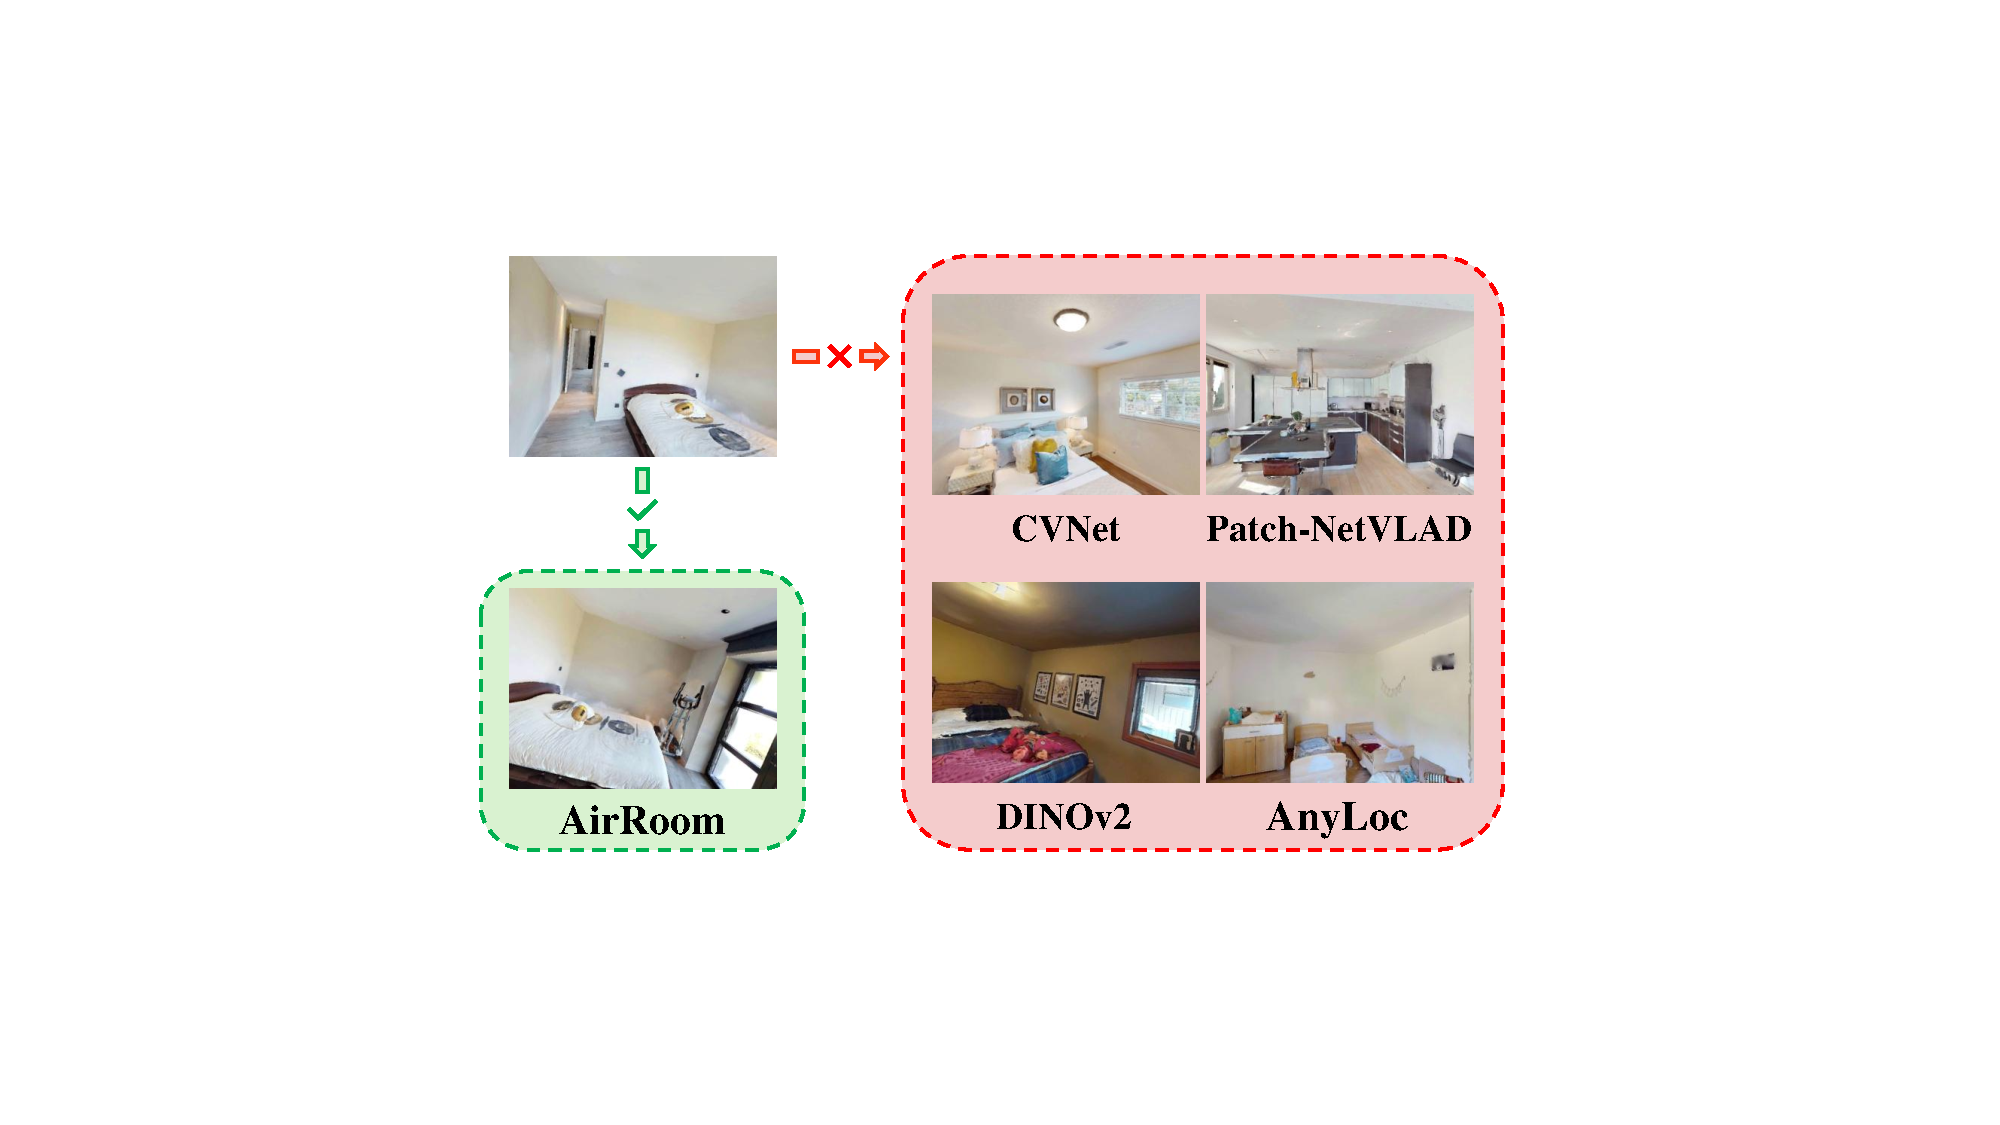
\includegraphics[width=\columnwidth]{failure_font.pdf}
    \vspace{-16pt}
    \caption{给定一个卧室查询,AirRoom 通过利用物体相关性进行房间重识别,准确地检索目标图像。相比之下,CVNet 检索视觉上相似的图像,但没有保持场景的准确性,DINOv2 捕捉语义内容但忽略了颜色细节,Patch-NetVLAD 使用聚合的局部特征形成全局描述符,检索到的图像语义信息不匹配,而 AnyLoc 考虑了语义和颜色属性,但忽略了房间内物体的重要性。}
    \vspace{-5pt}
    \label{fig:failure}
\end{figure}

\tref{tab:overall} 展示了 AirRoom 与基线方法之间的定量比较,结果表明 AirRoom 在几乎所有指标和数据集上均优于所有基线方法。在房间重识别任务中,图像检索方法由于其并非专注于 top-1 精度,通常在分类指标上表现较差,而 VPR 方法则取得了更好的结果。基于全局描述子的 VPR 方法仅捕捉高层语义信息,常常检索到语义相似但缺乏细节的房间;相比之下,使用局部特征聚合的 VPR 方法(如 Patch-NetVLAD)强调低层编码,但可能忽视全局上下文,从而导致检索准确性下降。 \fref{fig:failure} 展示了 CVNet、DINOv2、Patch-NetVLAD 和 AnyLoc 的失败案例,突显了这些方法的局限性。

尽管 AnyLoc 因其在“任何位置、任何时间、任何视角” VPR 中表现稳健而著称,并具有良好性能,但 AirRoom 进一步提升了表现,在可用提升空间内相较 AnyLoc 提高了 20\% 到 40\%。例如,AnyLoc 在 HMReID 上取得了 89.69\% 的准确率,留下了约 10\% 的提升空间;而 AirRoom 凭借 93.80\% 的准确率,在剩余空间内实现了高达 40\% 的提升。这些结果突显了 AirRoom 在房间重识别任务中卓越的精度与优化表现。
\subsection{按组别的性能比较}
\label{sec:section4.5}
\vspace{-3pt}
许多基准方法采用“骨干网络 + 增强机制”的范式,我们的方法也遵循这一范式。在本节中,我们将使用与每个组基准相同的骨干网络,将我们的面向对象增强机制与几种最先进的方法进行性能比较。此设置使我们能够直接评估我们的面向对象增强机制的有效性。

对于ResNet50骨干网络组,我们使用CVNet \cite{lee2022correlationverificationimageretrieval} 作为基准。在NetVLAD骨干网络组中,我们采用Patch-NetVLAD \cite{hausler2021patchnetvladmultiscalefusionlocallyglobal} 作为基准,并在三种降维度下进行测试:4096、512和128。

\tref{tab:grouped}显示,在每个组别中,单一的骨干网络优于那些通过各种机制尝试增强性能的基准方法,这表明这些机制未能有效地捕捉到室内环境中的关键信息。相比之下,我们的面向对象增强机制通过强调室内环境中\mbox{对象}的重要性,显著提升了骨干网络的性能。
\subsection{管道灵活性评估}  
\label{sec:section4.6}  
\vspace{-3pt}  
在本节中,我们通过测试其关键模块的不同配置,系统性地评估了 AirRoom 的灵活性和适应性。结果清楚地表明,AirRoom 并不依赖于任何特定模型,能够有效集成各种不同类型的模型。  

\vspace{-5pt}
\subsubsection{全局特征提取器}
\vspace{-4pt}
我们测试了多种全局特征提取器,包括ViT \cite{dosovitskiy2021imageworth16x16words}、DINO \cite{caron2021emergingpropertiesselfsupervisedvision}、DINOv2 \cite{oquab2024dinov2learningrobustvisual} 和AnyLoc-VLAD-DINOv2 \cite{keetha2023anylocuniversalvisualplace},VLAD簇大小分别为16和8。

如\tref{tab:global feature extractor flexibility}所示,AirRoom在几乎所有情况下,在所有度量标准和数据集上始终能够超过85\%,无论使用的全局特征提取器的能力如何。即使是在DINOv2的唯一例外情况下,AirRoom的表现仍然提高了近15\%。这表明我们的管道的有效性并不依赖于任何特定的全局特征提取器,突显了AirRoom在各种主干配置下的适应性,并强调了其强大的灵活性。

\vspace{-5pt}
\subsubsection{实例分割}
\vspace{-4pt}
我们将传统的实例分割方法(如 Mask R-CNN \cite{he2018maskrcnn})与更近期的 approaches,包括 Semantic-SAM \cite{li2023semanticsamsegmentrecognizegranularity} 进行比较,后者利用先进技术实现更细粒度的分割。

\tref{tab:is flexibility} 显示,无论使用何种实例分割模块,AirRoom 始终比基准方法高出超过 15\%。这证明了我们的管道不依赖于任何特定的实例分割方法,强调了其在此组件中的适应性。

\begin{table}[h]
\vspace{-5pt}
\centering
\resizebox{\columnwidth}{!}{
\begin{tabular}{l|cccc}
\toprule
\multirow{2}{*}{\textbf{Methods}} & \multicolumn{4}{c}{\textbf{HMReID}} \\
 & Accuracy & Precision & Recall & F1 \\
\midrule
DINOv2 & 53.91 & 60.52 & 53.73 & 54.69 \\
\rowcolor{Lavender} AirRoom-MaskRCNN & 69.44 & 72.23 & 69.08 & 69.07 \\
\rowcolor{Lavender} AirRoom-SSAM & \textbf{70.95} & \textbf{73.86} & \textbf{70.66} & \textbf{70.78} \\
\bottomrule
\end{tabular}
}
\vspace{-10pt}
\caption{实例分割的灵活性。}
\vspace{-16pt}
\label{tab:is flexibility}
\end{table}
\subsubsection{目标特征提取器}

我们实验了传统的骨干网络,如 ResNet50 \cite{he2015deepresiduallearningimage},以及更现代的骨干网络,如 DINOv2 \cite{oquab2024dinov2learningrobustvisual},作为目标特征提取器。

如 \tref{tab:ofe flexibility} 所示,AirRoom 在基准模型上实现了显著的性能提升,不同目标特征提取器之间的性能变化很小。这支持了我们管道在适应各种特征提取方法方面的灵活性。

\begin{table}[h]
\vspace{-6pt}
\centering
\resizebox{\columnwidth}{!}{
\begin{tabular}{l|cccc}
\toprule
\multirow{2}{*}{\textbf{Methods}} & \multicolumn{4}{c}{\textbf{HMReID}} \\
 & Accuracy & Precision & Recall & F1 \\
\midrule
DINOv2 & 53.91 & 60.52 & 53.73 & 54.69 \\
\rowcolor{Lavender} AirRoom-ResNet50 & \textbf{70.95} & \textbf{73.86} & \textbf{70.66} & \textbf{70.78} \\
\rowcolor{Lavender} AirRoom-DINOv2 & 68.67 & 71.81 & 68.33 & 68.59 \\
\bottomrule
\end{tabular}
}
\vspace{-10pt}
\caption{目标特征提取器的灵活性。}
\vspace{-20pt}
\label{tab:ofe flexibility}
\end{table}
\subsubsection{面向对象评分}

我们评估了均值 (\(s_{\text{mean}}\)) 和最大值 (\(s_{\max}\)) 两种策略,用于计算补丁得分 (\(s_{\text{patch}}\)) 和对象得分 (\(s_{\text{object}}\)),并评估它们对整体性能的影响。

\tref{tab:os flexibility} 显示,无论使用何种面向对象的评分方法,AirRoom的性能保持稳定。这突显了面向对象信息在房间重新识别中的稳健性,并展示了AirRoom在适应不同评分策略方面的灵活性。

\begin{table}[h]
\vspace{-6pt}
\centering
\resizebox{\columnwidth}{!}{
\begin{tabular}{l|cccc}
\toprule
\multirow{2}{*}{\textbf{Methods}} & \multicolumn{4}{c}{\textbf{HMReID}} \\
 & Accuracy & Precision & Recall & F1 \\
\midrule
DINOv2 & 53.91 & 60.52 & 53.73 & 54.69 \\
\rowcolor{Lavender} AirRoom-Max(patch)-Mean(object) & 70.95 & 73.86 & 70.66 & 70.78 \\
\rowcolor{Lavender} AirRoom-Max(patch)-Max(object) & \textbf{71.02} & \textbf{74.02} & \textbf{70.72} & \textbf{70.85} \\
\rowcolor{Lavender} AirRoom-Mean(patch)-Max(object) & 70.85 & 73.85 & 70.55 & 70.70 \\
\rowcolor{Lavender} AirRoom-Mean(patch)-Mean(object) & 70.90 & 73.78 & 70.62 & 70.73 \\
\bottomrule
\end{tabular}
}
\vspace{-10pt}
\caption{面向对象的评分灵活性。}
\vspace{-20pt}
\label{tab:os flexibility}
\end{table}
\subsection{消融研究}
\label{sec:section4.7}

在本节中,我们从我们的管道中移除某些模块——包括全局得分 \(s_{\text{global}}\)、局部得分 \(s_{\text{patch}}\)、目标得分 \(s_{\text{object}}\)(在目标感知评分中)以及整个细粒度检索(FGR)——以评估每个组件的重要性和有效性。

\begin{table}[t]
\centering
\resizebox{\columnwidth}{!}{
\begin{tabular}{l|cccc}
\toprule
\multirow{2}{*}{\textbf{Methods}} & \multicolumn{4}{c}{\textbf{HMReID}} \\
 & Accuracy & Precision & Recall & F1 \\
\midrule
DINOv2 (AirRoom-w/o all)& 53.91 & 60.52 & 53.73 & 54.69 \\
\rowcolor{Lavender} AirRoom-w/o \(s_{\text{patch}}\) & 66.68 & 70.04 & 66.42 & 66.68 \\
\rowcolor{Lavender} AirRoom-w/o \(s_{\text{object}}\) & 69.77 & 72.84 & 69.48 & 69.64 \\
\rowcolor{Lavender} AirRoom-w/o FGR & 66.11 & 70.85 & 65.80 & 66.41 \\
\rowcolor{Lavender} AirRoom-w/o \(s_{\text{patch}}\) \& \(s_{\text{object}}\) & 62.26 & 66.43 & 62.03 & 62.46 \\
\rowcolor{Lavender} AirRoom-w/o \(s_{\text{patch}}\) \& FGR & 59.39 & 65.25 & 59.14 & 59.97 \\
\rowcolor{Lavender} AirRoom-w/o \(s_{\text{object}}\) \& FGR & 63.44 & 68.68 & 63.14 & 63.84 \\
\rowcolor{Lavender} AirRoom & \textbf{70.95} & \textbf{73.86} & \textbf{70.66} & \textbf{70.78} \\
\bottomrule
\end{tabular}
}
\vspace{-10pt}
\caption{消融研究(不包括全局评分实验)。}
\vspace{-6pt}
\label{tab:ablation w/o global score}
\end{table}

\begin{table}[ht]
\centering
\resizebox{\columnwidth}{!}{
\begin{tabular}{l|cccc}
\toprule
\multirow{2}{*}{\textbf{Methods}} & \multicolumn{4}{c}{\textbf{HMReID}} \\
 & Accuracy & Precision & Recall & F1 \\
\midrule
ViT & 76.47 & 79.37 & 76.04 & 75.91 \\
\rowcolor{Lavender} AirRoom-ViT-w/o \(s_{\text{global}}\) & 84.86 & 86.82 & 84.34 & 84.61 \\
\rowcolor{Lavender} AirRoom-ViT & \textbf{86.58} & \textbf{88.13} & \textbf{86.12} & \textbf{86.23} \\
\cdashline{1-5}
DINOv2 & 53.91 & 60.52 & 53.73 & 54.69 \\
\rowcolor{Lavender} AirRoom-DINOv2-w/o \(s_{\text{global}}\) & \textbf{71.73} & \textbf{74.97} & \textbf{71.44} & \textbf{71.64} \\
\rowcolor{Lavender} AirRoom-DINOv2 & 70.95 & 73.86 & 70.66 & 70.78 \\
\bottomrule
\end{tabular}
}
\vspace{-10pt}
\caption{关于全局得分的消融研究。}
\vspace{-15pt}
\label{tab:ablation on global score}
\end{table}

\tref{tab:ablation w/o global score} 显示,移除任何模块都会导致性能下降。然而,只要至少保留一个模块,我们的管道仍然优于基线。 \tref{tab:ablation on global score} 证明,当全局特征提取器(ViT)表现良好时,全局得分 \(s_{\text{global}}\) 显著提升性能。另一方面,当全局特征提取器(DINOv2)效果较差时,全局得分 \(s_{\text{global}}\) 会产生轻微的负面影响,导致性能略微下降。这个结果与我们在第~\ref{subsec:refinement}节中的假设一致,其中全局得分充当优先级排序的先验,用于排名五个候选者的优先级。总体而言,这些消融研究确认了我们管道中的每个模块都是重要且必要的。
\subsection{局限性}

尽管AirRoom在不同视角变化下的房间重识别任务中达到了最先进的性能,但我们工作的一个局限性是无法验证其对由可移动物体引起的室内物品重排的鲁棒性。尽管我们基于互最近邻的物体感知评分方法在一定程度上对这种重排具有鲁棒性,但我们实验中使用的数据集缺乏这些情况。相比之下,最近在动态场景理解方面的进展 \cite{zhao2024dynamicsceneunderstandingobjectcentric} 专注于在存在移动物体的情况下识别场景,可能比我们的方法提供更强的鲁棒性。未来的工作应考虑构建包含物体重排的数据集,并集成新技术以增强对可移动物体的鲁棒性,从而提高房间重识别的性能。
